\documentclass{article}
\usepackage{array}
\usepackage{etoolbox}
\usepackage{fancyhdr}
\usepackage{geometry}
\usepackage{graphicx}
\usepackage{soul}
\usepackage{titling}
\usepackage[english]{babel}
\usepackage[backend=biber]{biblatex}
\addbibresource{references.bib}
\usepackage{geometry}
\usepackage{float}
\usepackage{tikz}
\usetikzlibrary{shapes.geometric, arrows}
\usepackage{hyperref}
\usepackage{pgfplots}

% Set the page margins as per your requirement
\geometry{
    top=1in,
    bottom=1in,
    left=0.65in, % Increase the left margin
    right=0.65in, % Increase the right margin
}

%%%%%%%%%%%%%%%%%%%%%%%%%%%%%%%%%%%%%%%%%%%%%%%%%%%%%%%%%%%%
% BEGIN METADATA: Edit the following as appropriate
%%%%%%%%%%%%%%%%%%%%%%%%%%%%%%%%%%%%%%%%%%%%%%%%%%%%%%%%%%%%

\title{Bill-E}%Illuminating Pakistan's Electricity Consumption and Billing*%  % the title of your project
\newcommand\shorttitle{\thetitle}  % if needed: a shorter title for the document header
% Team members.
\newcommand\firstname{Ali Asghar Yousuf}  % full name
\newcommand\firstid{ay06993}         % ID, e.g. xy01234
\newcommand\secondname{Muhammad Azeem Haider} % full name
\newcommand\secondid{mh0658}        % ID, e.g. xy01234
\newcommand\thirdname{Mohammad Shahid Mahmood}  % full name
\newcommand\thirdid{mm06600}         % ID, e.g. xy01234
% Uncomment the rows for the next 2 students if and as needed.
\newcommand\fourthname{Syed Ibrahim Ali Haider} % full name
\newcommand\fourthid{sh06565}        % ID, e.g. xy01234
% \newcommand\fifthname{Student 5}  % full name
% \newcommand\fifthid{id05}         % ID, e.g. xy01234

%%%%%%%%%%%%%%%%%%%%%%%%%%%%%%%%%%%%%%%%%%%%%%%%%%%%%%%%%%%%
% END METADATA: Do not edit the preamble any further.
%%%%%%%%%%%%%%%%%%%%%%%%%%%%%%%%%%%%%%%%%%%%%%%%%%%%%%%%%%%%

\pagestyle{fancy}
\lhead{SRS}
\chead{\shorttitle}
\rhead{Fall 2023}
\cfoot{Page \thepage}
\renewcommand{\footrulewidth}{0.4pt}

\newcommand\instruction[1]{\textit{#1}}

\begin{document}

% Cover page.
\begin{titlepage}

\center % Center everything on the page
 
%----------------------------------------------------------------------------------------
%	HEADING SECTIONS
%----------------------------------------------------------------------------------------

\textsc{
  {\LARGE \bf \thetitle}\\\bigskip\bigskip % Your Project Title
  {\large
    Kaavish Software Requirements Specification\\\bigskip
    By}
}\\\bigskip 

%----------------------------------------------------------------------------------------
%	AUTHOR SECTION
%----------------------------------------------------------------------------------------

{\large
  \begin{tabular}{ll}
    \firstname & (\firstid@st.habib.edu.pk) \\
    \secondname & (\secondid@st.habib.edu.pk) \\
    \thirdname & (\thirdid@st.habib.edu.pk) \\
    \ifdef{\fourthname}{\fourthname & (\fourthid@st.habib.edu.pk) \\}{}
    \ifdef{\fifthname}{\fifthname & (\fifthid@st.habib.edu.pk) \\}{}
  \end{tabular}
}
\bigskip\bigskip\bigskip

{\large \today}\\\bigskip\bigskip


\includegraphics[height=5cm]{HU_logo}\\\bigskip
 
%----------------------------------------------------------------------------------------
{\large
  In partial fulfillment of the requirement for \\\medskip
Bachelor of Science \\\medskip
Computer Science
}\\\bigskip\bigskip\bigskip

{\large
  \textsc{
    Dhanani School of Science and Engineering\\\bigskip
    Habib University\\\bigskip 
    Fall 2023
  }\\\bigskip\bigskip 
  Copyright @ 2023 Habib University
}

\end{titlepage}


\tableofcontents
\newpage

%%%%%%%%%%%%%%%%%%%%%%%%%%%%%%%%%%%%%%%%%%%%%%%%%%%%%%%%%%%%
% DATA: Populate the rest of the document as instructed.
%%%%%%%%%%%%%%%%%%%%%%%%%%%%%%%%%%%%%%%%%%%%%%%%%%%%%%%%%%%%
\section{Introduction}
This Software Requirements Specification (SRS) Document is a blueprint for the
development of our final year project's product, Bill-E, a mobile application
to calculate electricity consumption that aims to serve the public with
insights about their electricity bill and the units they consume over the
course of a specified period. This document will outline the project plan,
including the goals and objectives. It will also delve deep into the functional
and non-functional requirements that we aim to meet whilst creating this
software solution. It is intended for all the various stakeholders including
the students, supervisors, testers, and end users, ensuring a common
understanding of the scope and the behavior of the software.

\subsection{Purpose}
The primary purpose of this SRS document is to define the functionality and
features of the software and have a set of requirements in order to guide the
development team. It will also help to plan, estimate, and allocate resources
effectively.

\subsection{Scope}
The scope of this document will cover the following key elements of Bill-E.
\begin{itemize}
    \item \textbf{Functionality and features:} A detailed description of the features and functionality of the application with a clear understanding of the software's expectations outlining the operations, interactions, and capabilities that the stakeholders may experience.
    \item \textbf{Requirements Guidance} This SRS document aims to establish an unambiguous set of requirements, which will serve as a guideline for the developers. These will include the functional and the non-functional requirements, as well as other important system requirements. All these are important for the designing, developing, and testing of the software.
    \item  \textbf{Project Planning and Resource Allocation:} By having a  clear set of requirements, the SRS document will aid the team in effectively planning the project and allocating the required resources.
\end{itemize}

\section{Project Plan}
This section is where the different goals and objectives of the project are
clearly stated and broken down into tasks. These tasks are then given a time
frame and they are allotted the required resources. It is essential to have a
project plan as it gives all the stakeholders, including student developers and
supervisors a clear outline of the timelines and deliverables. An added part in
this section is the risks that are involved in all the various parts of the
development journey of the project.

\subsection{Objectives}

\begin{itemize}
    \item \textbf{Project Goals:} The main goal of this project is to create a software solution that serves as a medium for Pakistanis, specifically from Karachi, to be able to predict their electricity consumption based on their usage patterns. In addition, the application aims to provide recommendations to the users to reduce their electricity bill units. Providing users with analytics of their usage serves as the secondary biggest goal of the software.
    \item \textbf{Deliverable:}
          \begin{itemize}
              \item Mobile Application: A fully functional mobile application tailored to the
                    Pakistani context, enabling electricity consumption prediction and billing
                    estimation.
              \item Prediction Model: An accurate predictive model that predicts the Household
                    electricity consumption and is integrated with the Mobile App.
              \item Optimization model: A model which able to provide suggestions and facts to
                    optimize electricity consumption to Users and is based on user inputs,
                    predictions from the prediction model, and few other variables
          \end{itemize}
    \item \textbf{Success Criteria:} The success criteria for Bill-E can be defined as follows:
          \begin{itemize}
              \item An intuitive and interactive mobile application with an easy-to-use UI/UX
                    keeping our target audience in mind.
              \item The Prediction Model is able to predict household consumption within a margin
                    of 7-10\% error.
              \item The Optimization Model is smart enough to understand the user's usage and is
                    able to suggest doable actions to optimize the electricity consumption of the
                    household.
              \item The analytics provided to the user proves to be helpful to the user to keep
                    track of the user's usage.
          \end{itemize}

\end{itemize}

\subsection{Tasks and Timeline}
\begin{itemize}
    \item \textbf{Initial data collection} 10 October - 25 October \\
          This Data is collected via a survey form to give the team a starting point and enable the website to give a prediction. This prediction is done with a Linear regression model
    \item \textbf{Website} 1 November - 25 November \\
          A Website is deployed with the intention of collecting data for the deep learning model.
    \item \textbf{Data manipulation/cleaning} 25 October - 30 November \\
          The initial data collected through surveys and the website is cleaned and manipulated to be used for the deep learning model.
    \item \textbf{Wire Frames - High Fidelity} Designs 1 November - 15 November \\
          Wire Frames are important as they give the team a good vision of what the front end of the app will appear
    \item \textbf{App Low Fidelity Frontend} 15 November - 30 November \\
          The initial frontend of the app is developed encompassing all the features and functionalities
    \item \textbf{Model Train} 15 November - 10 January \\
          The model is trained on the data collected from the website and the survey

    \item \textbf{Backend/API Development} 30 November - 10 January \\
          The backend of the app is developed to enable the app to interact with the database and the model

    \item \textbf{Recommendation System} 15 November - 10 January \\
          The recommendation system will power the analytics tab of the app and will be able to provide suggestions to the user to optimize their electricity consumption
    \item \textbf{App High Fidelity Frontend} 10 January - 15 February \\
          The final frontend of the app is developed encompassing all the features and functionalities
    \item \textbf{App Testing} 15 January - 15 February, 1 March - 15 March \\
          The App will be tested in two phases, the first phase will be to test the design and UI/UX of the app and the second phase will be to test the functionality of the app
    \item \textbf{Integration} 5 February - 28 February \\
          The model, the backend, the frontend, and the recommendation system are integrated to form the final product

\end{itemize}
% \subsection{Timeline}

% \begin{itemize}
%     \item Project Schedule:
%     \item Milestones:
%     \item 
% \end{itemize}
\subsection{Risks}
The risks involved with this project are as follows:
\begin{itemize}
    \item The data collection process for the prediction model is not successful and
          augmented data is used to a large extent.
    \item The introduction of the augmented data would mean compromising on the accuracy
          of the prediction model which is central to our project.
    \item The solution caters to a specific Socio-economic group rendering it useless to
          the large masses which are the most impacted when it comes to electricity bill
          hikes.
\end{itemize}

\section{Software Requirements Specification}
\subsection{Functional Requirements}
Functional Requirements are a category of software requirements that describe
what a software system or application is expected to do focusing on the
interaction between the systems. These requirements detail the specific actions
the software should be able to perform. this includes the inputs and the
outputs, data processing, and user interface. They are essential for the design
and development of the software. Following are the main functions of our
software, Bill-E.
\subsubsection{Profile Management}
\begin{enumerate}
    \item \textbf{User Registration and Deletion}
          \begin{itemize}
              \item Users can create an account with personal information
              \item Users can delete their accounts if necessary
          \end{itemize}

    \item \textbf{Room Breakdown}
          \begin{itemize}
              \item Users will define rooms within their house and their structure.
              \item User can add or remove rooms.
          \end{itemize}
    \item \textbf{Appliances Management}
          \begin{itemize}
              \item Users can add and remove heavy, in-use appliances and specify their usage
                    hours.
              \item Users can update the appliances and their usage hours.
          \end{itemize}
    \item \textbf{Past Billing Information}
          \begin{itemize}
              \item Users will input usage units for past months to enhance energy consumption
                    predictions.
          \end{itemize}

    \item \textbf{User Profile Update}
          \begin{itemize}
              \item Users can edit and update their profile information.
          \end{itemize}

\end{enumerate}

\subsubsection{Electricity Consumption Forecast}
\begin{enumerate}
    \item \textbf{Predicted Electricity Consumption}
          \begin{itemize}
              \item Users receive predictions, in units, for their overall electricity consumption
                    based on the provided usage data.
          \end{itemize}

    \item \textbf{Predicted Room Consumption}
          \begin{itemize}
              \item Users receive predictions, in units, for room-wise electricity consumption
                    patterns based on the provided data.
          \end{itemize}

    \item \textbf{Predicted Bill}
          \begin{itemize}
              \item Users receive predictions for their electricity bills based on the provided
                    usage data.
          \end{itemize}
\end{enumerate}

\subsubsection{Electricity Conversation Patterns}
Users will get the optimal electricity usage pattern, according to their
household information.

\subsubsection{Analytics}
Users can access various analytics related to their electricity consumption.

\begin{enumerate}
    \item \textbf{Highest Room Usage}
          \begin{itemize}
              \item Users can view the room that has consumed the most electricity.
          \end{itemize}

    \item \textbf{Highest Usage Appliance}
          \begin{itemize}
              \item Users can identify the appliance that has consumed the most electricity.
          \end{itemize}

    \item \textbf{Peak Consumption Time}
          \begin{itemize}
              \item Users can determine their peak electricity consumption time.
          \end{itemize}

    \item \textbf{Electricity Conservation Tips}
          \begin{itemize}
              \item Users can access and view various tips/facts for conserving electricity.
          \end{itemize}

    \item \textbf{Bill Alerts}
          \begin{itemize}
              \item Users will receive alerts if their electricity usage is projected to exceed a
                    specific threshold just above the current slab rate.
          \end{itemize}
\end{enumerate}

\subsection{Non-Functional Requirements}
Our app aims for the following non-functional requirements:
\subsubsection{Performance and Robustness}
The app should run smoothly. The prediction step should respond within 5-7
seconds. The app should be able to handle a large number of users. The API
should be able to handle at least 100 requests per minute.

\subsubsection{Security}
User data should be secure and one user's data should not be accessible to
another user. Sensitive data such as passwords should be encrypted. The user
data should not be accessible by a third party.

\subsubsection{Usability}
The app should have an intuitive UI. People of every age group should be able
to navigate through the app without much help.

\subsubsection{Compatibility}
The app should be compatible with both Android and iOS devices.

\subsubsection{Data Storage and Retention}
Ensure that the data collected is organized and stored in a secure manner. The
data retrieval should be streamlined. The data is backed up and can be restored
in case of any data loss.

\subsubsection{Scalability}
The app should be deployed on a scalable platform. The app should be able to
handle a large number of users and should be able to scale up or down according
to the number of users.

\subsubsection{Compliance}
The app should comply with the laws and regulations of Pakistan. The app should
comply with the privacy laws of Pakistan.

\subsubsection{Reliability}
The app should be reliable and should be equipped to handle any errors that may
occur. The app should be able to handle any errors gracefully and should not
crash.

\subsection{Usecase Diagram and Description}

\begin{figure}[H]
    \centering
    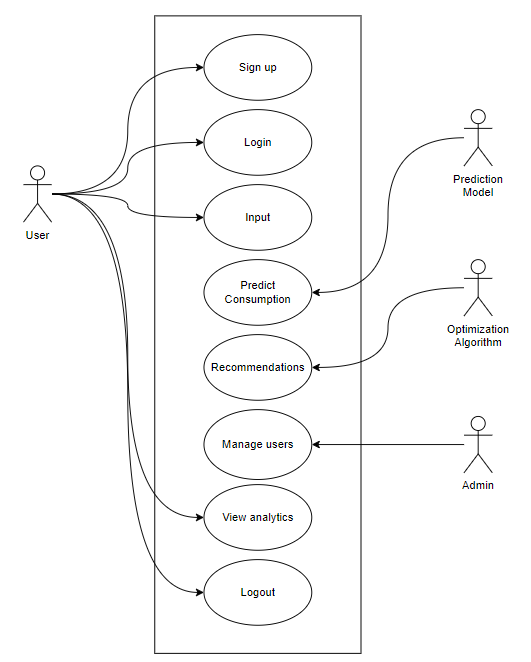
\includegraphics[width=0.6\textwidth]{images/usecase.png}
    \caption{Use Case Diagram}
    \label{fig: Use Case Diagram}
\end{figure}

\subsubsection{Description:} The use case diagram serves the important purpose of visually giving a basic
rundown of how the App will function for different Stakeholders. The Box
indicates the boundary of the Applications and objects within the box are
basically functional requirements of the application shown visually.
\begin{itemize}
    \item \textbf{Purpose: } The purpose of this Use case Diagram is to give an overview of all the Actors and how the interaction with the software will look like. The Use case diagram acts like a visual tool that gives a topological perspective of all different types of interactions and relationships.
    \item \textbf{Actors:} Actors are all the external entities involved in the operations of the App. In our Use case diagram, we have 4 different actors.
          \begin{itemize}
              \item The user: The user is the primary Actor of the application. they will interact
                    will all the different features in the App. They will provide inputs, be able
                    to see the analytics, sign up, log in, and log out.
              \item The Admin: Admin will be the Actors who will only be responsible for the
                    management of the users.
              \item Predictive Model: It will be the Main model which will be trained and here is
                    where the forecasted/ predicted results of the electricity consumption will
                    come from.
              \item Optimization Algorithm: This will be the added model/Algorithm that will be
                    responsible for recommending different actions to users in order to make their
                    electricity consumption as optimal as possible.
          \end{itemize}
    \item \textbf{Use Cases:} Use cases represent all the various functionalities of the software. Each use case represents its specified interaction
    \item \textbf{Associations:} The associations are represented by arrows, that simply signify an interaction between an actor and the use case.
    \item \textbf{System Boundary:} The system boundary visually shows which parts of the entire interactive experience lie within the system and which lie outside.
\end{itemize}

\subsection{System Diagram and Description:}

\begin{figure}[H]
    \centering
    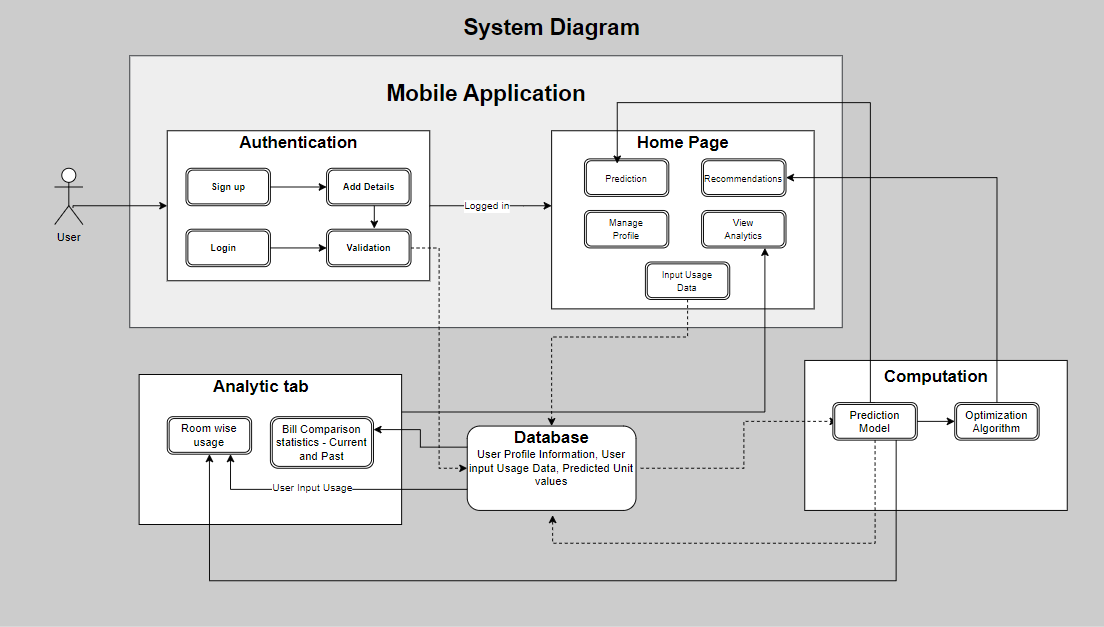
\includegraphics[width=0.8\textwidth]{images/system.png}
    \caption{Use Case Diagram}
    \label{fig: System Diagram}
\end{figure}

\subsubsection{Description}
The system diagram illustrates the various interfaces of the final design of
our project, which consists of four main components:

\begin{enumerate}
    \item Mobile Application
    \item Analytic tab
    \item Database
    \item Computational Models
\end{enumerate}

The mobile application is the primary component through which users will
interact with the system. Initially, users will be prompted to sign up or log
in to the application. User credentials will be authenticated, as security is a
critical non-functional requirement for our mobile application. After
successful login, first-time users will be asked to provide data on their
appliance usage to predict their electricity bill based on subsequent usage.
The prediction model will use this usage data to forecast electricity
consumption. Subsequently, an optimization plan for the user's electricity
usage will be provided based on the predicted units. Additionally, users will
have access to analytics, allowing them to review their electricity consumption
for the previous month and analyze room-wise electricity usage.

Users revisiting the application will be able to view their analytics and the
optimization plan provided to them previously to reduce their electricity bill.
In addition, users at all times will have the power to change their usage
patterns, since the patterns will be different for each season based on
different factors. Once the user usage data is updated, the prediction model
will calculate the units based on the newly inputted usage data.

\section{Software Design Specifications}
\subsection{System Architecture}
The system architecture is the structural design of the software system. It
includes the software components, the externally visible properties of those
components, and the relationships among them. The system architecture serves as
a blueprint for the system and the developers. It is essential to have a system
architecture as it gives a clear understanding of the system and its
components. It also helps in the development of the system as it gives a
clearer picture of the system and its components. The system architecture of
our software, Bill-E, is as follows:

\begin{figure}[H]
    \centering
    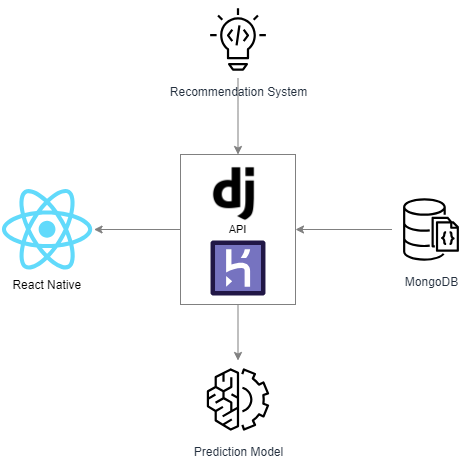
\includegraphics[width=0.6\textwidth]{images/architecture.png}
    \caption{System Architecture}
    \label{fig: System Architecture}
\end{figure}

\subsubsection{Backend}
There are four main components of the backend of our software. The first
component is the database. The database is where all the data is stored

\subsection{Database Design}
The database design is the process of producing a detailed data model of a
database. This data model contains all the needed logical and physical design
choices and physical storage parameters needed to generate a design. The
database design is essential as it helps in the development of the database and
the database management system. The database design of our software, Bill-E, is
as follows:

\begin{figure}[H]
    \centering
    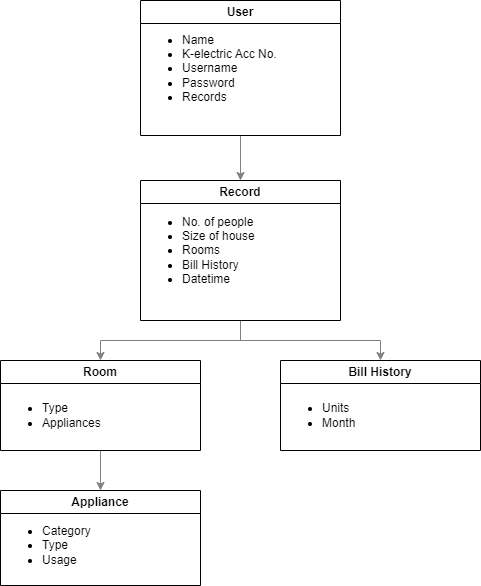
\includegraphics[width=0.8\textwidth]{images/data.png}
    \caption{Database Design}
    \label{fig: Database Design}
\end{figure}

\subsection{User Interface Design}

\printbibliography

% External advisor undertaking.
%\begin{titlepage}

  \newcolumntype{C}[1]{>{\centering\arraybackslash\hspace{0pt}}p{#1}}

  \centerline{\textbf{\ul{Undertaking of Kaavish advisement as an External Supervisor}}}
  \bigskip\bigskip

  I hereby affirm that I have read the project details as described on the preceding pages and agree to undertake advisement of this Kaavish project as an External Supervisor. I understand that this role entails the following.
  \begin{description}
  \item[Meeting] Meeting the project team regularly, at least once every two weeks, for the entire duration of the Kaavish. The meetings may be held remotely if required.
  \item[Advisement] Providing supervision and advice to the team in order to ensure steady progress of the project toward its goals.
  \item[Liaison] Liaising with the Internal Supervisor as required, e.g. to provide feedback or engage in grading.
  \item[Other] Any other task, depending on availability and suitability, relevant to the Kaavish as communicated by the Internal Supervisor or Kaavish Working Group.
  \end{description}

  \bigskip\bigskip\bigskip
  
  \noindent
  \begin{tabular}{@{}lp{.4\textwidth}}
    Name: & \hrulefill\\\\
    Email: & \hrulefill\\\\
    Phone: & \hrulefill\\\\
    Designation: & \hrulefill\\\\
    Affiliation: & \hrulefill\\\\\\
    Signature: & \hrulefill\\
  \end{tabular}
\end{titlepage}


\end{document}

%%% Local Variables:
%%% mode: latex
%%% TeX-master: t
%%% End:
